%%%%%%%%%%%%%%%%%%%%%%%%%%%%%%%%%%%%

\section{カイ二乗適合度検定}

%%%%%%%%%%%%%%%%%%%%%%%%%%%%%%%%%%%

\subsection{ウェルドンのサイコロ}

%%%%%%%%%%%%%%%%%%%%%%%%%%%%%%%%%%%

\begin{frame}
\frametitle{ウェルドンのサイコロ}

\twocol{0.75}{0.25}
{
\begin{itemize}

\item ウォルター・フランク・ラファエル・ウェルドン（1860--1906）は、イギリスの進化生物学者で、生物測定学の創設者の一人です。フランシス・ゴールトンおよびカール・ピアソンとともに、Biometrikaの共同創設編集者でした。

\item 1894年に、彼は12個のサイコロを26,306回振り、5か6が出た回数（成功とみなした）を記録しました。

\end{itemize}
}
{
\begin{center}
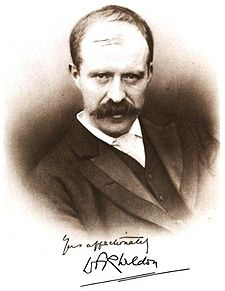
\includegraphics[width=\textwidth]{6-3_chisq_gof/figures/dice/weldon}
\end{center}
}
\begin{itemize}

\item 5か6が期待よりも頻繁に出ることが観察され、ピアソンはこれがサイコロの構造によるものだと仮説を立てました。安価なサイコロの多くは凹んだ点を持ち、反対の面の合計が7になるため、6の目のある面は1の目のある反対の面より軽くなります。

\end{itemize}

\end{frame}

%%%%%%%%%%%%%%%%%%%%%%%%%%%%%%%%%%%

\begin{frame}
\frametitle{ラビーのサイコロ}

\twocol{0.6}{0.4}
{
\begin{itemize}

\item 2009年、ザカライア・ラビー（シカゴ大学）は、手製のサイコロ投げ・点数カウント機械を使ってウェルドンの実験を再現しました。
\begin{center}
\webURL{http://www.youtube.com/watch?v=95EErdouO2w}
\end{center}

\item 転がして画像処理するのに約20秒かかりました。

\end{itemize}
}
{
\begin{center}
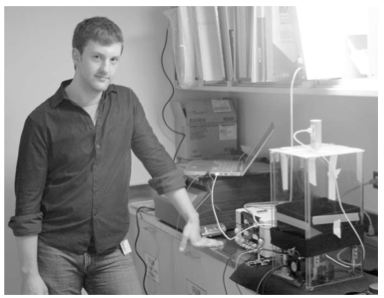
\includegraphics[width=\textwidth]{6-3_chisq_gof/figures/dice/labby}
\end{center}
}

\begin{itemize}

\item 1日あたり約150枚の画像を手動で処理する必要がありました。

\item このペースで、ウェルドンの実験は6日以上かけて再現されました。

\item 推薦読書：\webURL{http://galton.uchicago.edu/about/docs/labby09dice.pdf}

\end{itemize}

\end{frame}

%%%%%%%%%%%%%%%%%%%%%%%%%%%%%%%%%%%

\begin{frame}
\frametitle{ラビーのサイコロ（続き）}

\begin{itemize}

\item ラビーは実際には、ウェルドンが観察した現象（5と6の頻度が高い）を観察しませんでした。

\item 自動化によりラビーは1894年のウェルドンよりも多くのデータを収集でき、「成功」と「失敗」を記録する代わりに、各サイコロの個別の目の数を記録しました。

\end{itemize}

\begin{center}
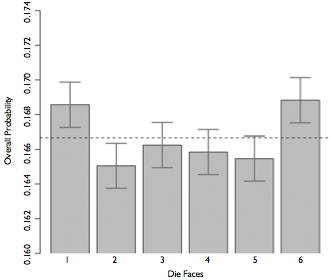
\includegraphics[width=0.5\textwidth]{6-3_chisq_gof/figures/dice/labbyPipCounts}
\end{center}

\end{frame}

%%%%%%%%%%%%%%%%%%%%%%%%%%%%%%%%%%%

\subsection*{一元表の検定統計量の作成}

%%%%%%%%%%%%%%%%%%%%%%%%%%%%%%%%%%%

\begin{frame}
\frametitle{期待度数}

\pq{ラビーは12個のサイコロを26,306回振りました。各面が等しい確率で出るとすれば、1、2、$\cdots$、6はそれぞれ何回出ることが期待されますか？}

\begin{enumerate}[(a)]
\item $\frac{1}{6}$
\item $\frac{12}{6}$
\item $\frac{26,306}{6}$
\solnMult{ $\frac{12 \times 26,306}{6}$ } \only<2->{\orange{$= 52,612$}}
\end{enumerate}

\end{frame}

%%%%%%%%%%%%%%%%%%%%%%%%%%%%%%%%%%%

\begin{frame}
\frametitle{ラビーの結果のまとめ}

以下の表は、ラビーの実験から得られた観測度数と期待度数を示しています。

{\small
\begin{center}
\renewcommand\arraystretch{1.2}
\begin{tabular}{c | c c}
結果	& 観測度数	& 期待度数 \\
\hline
1		& 53,222		& 52,612 \\
2		& 52,118		& 52,612 \\
3		& 52,465		& 52,612 \\
4		& 52,338		& 52,612 \\
5		& 52,244		& 52,612 \\
6		& 53,285		& 52,612 \\
\hline
合計		& 315,672		& 315,672
\end{tabular}
\end{center}
}

\dq{期待度数がすべての結果で同じなのに、観測度数が異なるのはなぜですか？一見して、観測度数と期待度数の間に不一致があるように見えますか？}

\end{frame}

%%%%%%%%%%%%%%%%%%%%%%%%%%%%%%%%%%%

\begin{frame}
\frametitle{仮説の設定}

\dq{これらのデータは、観測度数と期待度数の間の不一致の説得力のある証拠を提供しますか？}

\begin{itemize}
\item[$H_0$:] 観測度数と期待度数の間に不一致はありません。\hlGr{観測度数は期待度数と同じ分布に従います。}

\item[$H_A$:] 観測度数と期待度数の間に不一致があります。\hlGr{観測度数は期待度数と同じ分布に\orange{従いません}。}サイコロを振ったときに出る面にバイアスがあります。
\end{itemize}

\end{frame}

%%%%%%%%%%%%%%%%%%%%%%%%%%%%%%%%%%%

\begin{frame}
\frametitle{仮説の評価}

\begin{itemize}

\item これらの仮説を評価するために、観測度数が期待度数からどれだけ異なるかを定量化します。

\item 標本変動（偶然）のみによって期待される値から大きく逸脱している場合、対立仮説の強い証拠となります。

\item これは\hl{適合度}検定と呼ばれ、観測データが期待される分布にどの程度適合しているかを評価します。

\end{itemize}

\end{frame}

%%%%%%%%%%%%%%%%%%%%%%%%%%%%%%%%%%%

\subsection{カイ二乗統計量}

%%%%%%%%%%%%%%%%%%%%%%%%%%%%%%%%%%%

\begin{frame}
\frametitle{検定統計量の構造}

\begin{itemize}

\item 検定統計量の一般的な形は
\[ \frac{\text{点推定値} - \text{帰無値}}{\text{点推定値のSE}} \]

\item この構造は以下の2つに基づいています：
\begin{enumerate}
\item 帰無仮説が真の場合の期待値と点推定値の差を特定し、
\item その差を点推定値の標準誤差で標準化する。
\end{enumerate}

これらの2つの考え方が、度数データの適切な検定統計量の構築に役立ちます。

\end{itemize}

\end{frame}

%%%%%%%%%%%%%%%%%%%%%%%%%%%%%%%%%%%

\begin{frame}
\frametitle{カイ二乗統計量}

度数を扱い、観測度数が期待度数からどれだけ離れているかを調べる場合、\hl{カイ二乗（$\chi^2$）統計量}と呼ばれる新しい検定統計量を使用します。

$\:$ \\

\formula{$\chi^2$統計量}
{
\[\chi^2 = \sum_{i = 1}^k \frac{(O - E)^2}{E} \qquad \text{ここで$k$ = セルの総数} \]
}

\end{frame}

%%%%%%%%%%%%%%%%%%%%%%%%%%%%%%%%%%%

\begin{frame}
\frametitle{カイ二乗統計量の計算}

\begin{center}
\renewcommand\arraystretch{1.8}
\begin{tabular}{c | c c | c}
結果	& 観測度数	& 期待度数 	& $\frac{(O - E)^2}{E}$\\
\hline
1		& 53,222		& 52,612 		& $\frac{(53,222 - 52,612)^2}{52,612} = 7.07$ \\
2		& 52,118		& 52,612 		& $\frac{(52,118 - 52,612)^2}{52,612} = 4.64$ \\
3		& 52,465		& 52,612 		& $\frac{(52,465 - 52,612)^2}{52,612} = 0.41$ \\
4		& 52,338		& 52,612 		& $\frac{(52,338 - 52,612)^2}{52,612} = 1.43$\\
5		& 52,244		& 52,612 		& $\frac{(52,244 - 52,612)^2}{52,612} = 2.57$\\
6		& 53,285		& 52,612 		& $\frac{(53,285 - 52,612)^2}{52,612} = 8.61$\ \\
\hline
合計		& 315,672		& 315,672		& 24.73
\end{tabular}
\end{center}

\end{frame}

%%%%%%%%%%%%%%%%%%%%%%%%%%%%%%%%%%%

\begin{frame}
\frametitle{なぜ二乗するのか？}


観測された結果と期待された結果の差を二乗することは2つのことをします：
\begin{itemize}
\item 二乗された標準化された差はすべて正になります。
\item すでに異常に見えた差は、二乗後にさらに大きくなります。
\end{itemize}

\vspace{1cm}

\dq{以前にこのようなことを見たことがありますか？}

\end{frame}

%%%%%%%%%%%%%%%%%%%%%%%%%%%%%%%%%%%

\subsection{カイ二乗分布と面積の求め方}

%%%%%%%%%%%%%%%%%%%%%%%%%%%%%%%%%%%

\begin{frame}
\frametitle{カイ二乗分布}

\begin{itemize}

\item 計算した$\chi^2$統計量が異常に高いかどうかを判断するために、まずその分布を説明する必要があります。

\item カイ二乗分布は\hl{自由度（df）}と呼ばれる1つのパラメータのみを持ち、これが分布の形状、中心、広がりに影響します。\\

\end{itemize}

$\:$ \\

\Remember{これまでに3つの他の連続分布を見てきました：
\begin{itemize}
\item[-] 正規分布：平均と標準偏差の2つのパラメータを持つ単峰で対称な分布
\item[-] t分布：自由度の1つのパラメータを持つ単峰で対称な分布
\item[-] F分布：分子の自由度（グループ間分散）と分母の自由度（グループ内分散）の2つのパラメータを持つ単峰で右に歪んだ分布
\end{itemize}
}

\end{frame}

%%%%%%%%%%%%%%%%%%%%%%%%%%%%%%%%%%%

\begin{frame}
\frametitle{}

\pq{次のうち誤りはどれですか？}

\begin{center}
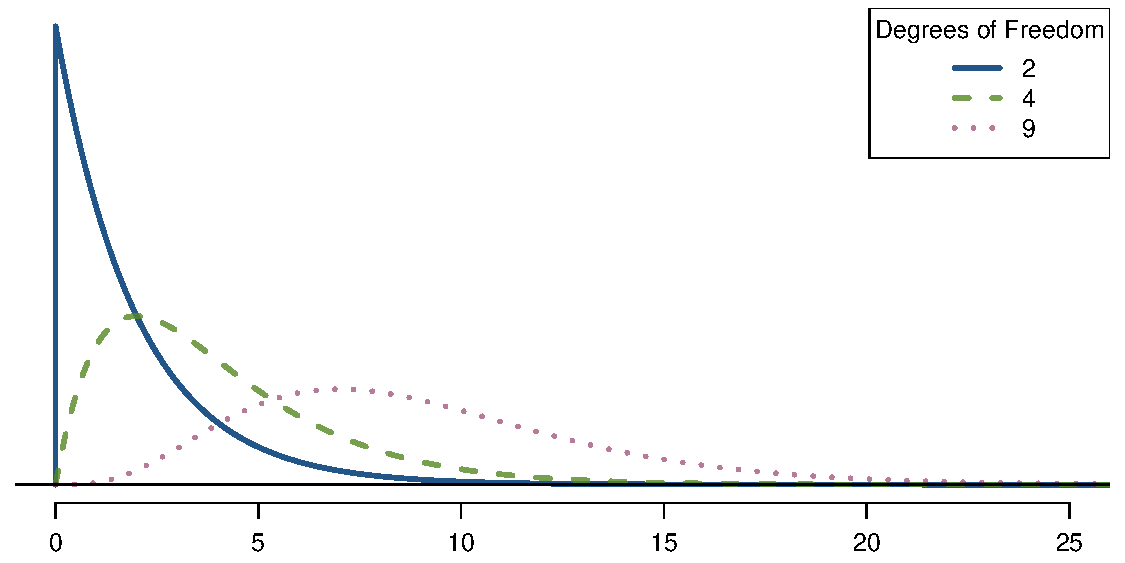
\includegraphics[width=0.7\textwidth]{6-3_chisq_gof/figures/chiSquareDistributionWithInceasingDF/chiSquareDistributionWithInceasingDF}
\end{center}

dfが増加するにつれて、
\begin{enumerate}[(a)]
\item $\chi^2$分布の中心も増加する
\item $\chi^2$分布のばらつきも増加する
\solnMult{$\chi^2$分布の形状がより歪んでくる（正規分布に近くなくなる）}
\end{enumerate}

\end{frame}

%%%%%%%%%%%%%%%%%%%%%%%%%%%%%%%%%%%

\begin{frame}[fragile]
\frametitle{カイ二乗曲線の下の面積を求める}

\begin{itemize}

\item p値 = カイ二乗分布の裾の面積（通常通り）

\item このためにテクノロジーやカイ二乗確率表を使用できます。

\end{itemize}

\end{frame}

%%%%%%%%%%%%%%%%%%%%%%%%%%%%%%%%%%%

\begin{frame}[fragile]
\frametitle{カイ二乗曲線の下の面積を求める（続き）}

\dq{$df = 6$の$\chi^2$曲線で、カットオフ値10より上の影付き部分の面積を推定してください。}

\begin{verbatim}

> pchisq(q = 10, df = 6, lower.tail = FALSE)

[1] 0.124652

\end{verbatim}

\end{frame}

%%%%%%%%%%%%%%%%%%%%%%%%%%%%%%%%%%%

\begin{frame}[fragile]
\frametitle{カイ二乗曲線の下の面積を求める（続き）}

\pq{$df = 9$の$\chi^2$曲線で、カットオフ値17より上の影付き部分の面積を推定してください。}

\twocol{0.6}{0.4}{
\begin{center}
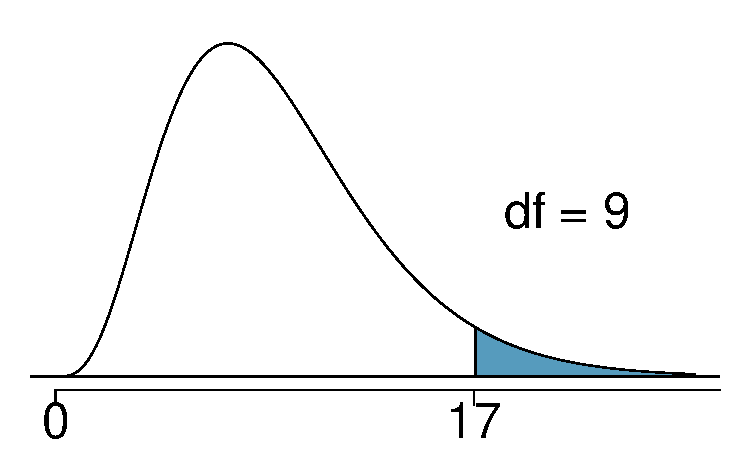
\includegraphics[width=0.67\textwidth]{6-3_chisq_gof/figures/above17WithDF9/above17WithDF9}
\end{center}
}
{
{\small
\begin{enumerate}[(a)]
\setlength{\itemsep}{0in}
\item 0.05
\item 0.02
\solnMult{0.02と0.05の間}
\item 0.05と0.1の間
\item 0.01と0.02の間
\end{enumerate}
}
}

\begin{verbatim}

> pchisq(q = 17, df = 9, lower.tail = FALSE)

[1] 0.04871598

\end{verbatim}

\end{frame}

%%%%%%%%%%%%%%%%%%%%%%%%%%%%%%%%%%%

\begin{frame}[fragile]
\frametitle{カイ二乗曲線の下の面積を求める（もう一問）}

\pq{$df = 10$の$\chi^2$曲線で、30より上の影付き部分の面積を推定してください。}

\twocol{0.6}{0.4}{
\begin{center}
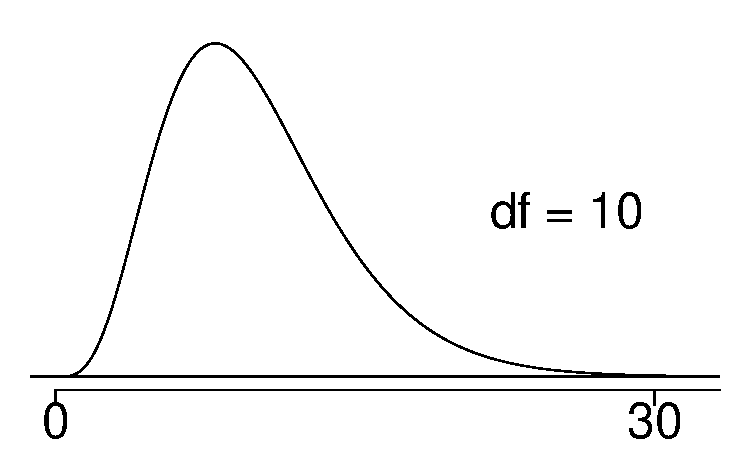
\includegraphics[width=0.67\textwidth]{6-3_chisq_gof/figures/above30WithDF10/above30WithDF10}
\end{center}
}
{
{\small
\begin{enumerate}[(a)]
\setlength{\itemsep}{0in}
\item 0.3より大きい
\item 0.005と0.001の間
\solnMult{0.001未満}
\item 0.001より大きい
\item この表では判断できない
\end{enumerate}
}
}

\begin{verbatim}

> pchisq(q = 30, df = 10, lower.tail = FALSE)

[1] 0.0008566412

\end{verbatim}

\end{frame}

%%%%%%%%%%%%%%%%%%%%%%%%%%%%%%%%%%%

\subsection{カイ二乗検定のp値の求め方}

%%%%%%%%%%%%%%%%%%%%%%%%%%%%%%%%%%%

\begin{frame}
\frametitle{ラビーのサイコロに戻ろう}

\begin{itemize}

\item 研究上の問いは：これらのデータは、観測度数と期待度数の間の不一致の説得力のある証拠を提供しますか？

\item 仮説は：
\begin{itemize}
\item[$H_0$:] 観測度数と期待度数の間に不一致はありません。観測度数は期待度数と同じ分布に従います。
\item[$H_A$:] 観測度数と期待度数の間に不一致があります。観測度数は期待度数と同じ分布に\orange{従いません}。サイコロを振ったときに出る面にバイアスがあります。
\end{itemize}

\item 検定統計量\orange{$\chi^2 = 24.67$}を計算しました。

\item $df$があれば、裾の面積（p値）を計算して仮説に関する決定を下すことができます。

\end{itemize}

\end{frame}

%%%%%%%%%%%%%%%%%%%%%%%%%%%%%%%%%%%

\begin{frame}
\frametitle{適合度検定の自由度}

\begin{itemize}

\item 観測データが期待される分布にどの程度適合しているかを評価する適合度検定では、自由度はセル数（$k$）から1を引いた値として計算されます。
\[ \mathhl{df = k - 1} \]

\item サイコロの結果では$k = 6$なので、
\[ df = 6 - 1 = 5 \]

\end{itemize}

\end{frame}

%%%%%%%%%%%%%%%%%%%%%%%%%%%%%%%%%%%

\begin{frame}
\frametitle{カイ二乗検定のp値の求め方}

カイ二乗検定の\hl{p値}は、\hl{計算された検定統計量より上の裾の面積}として定義されます。

\twocol{0.6}{0.4}{
\begin{center}
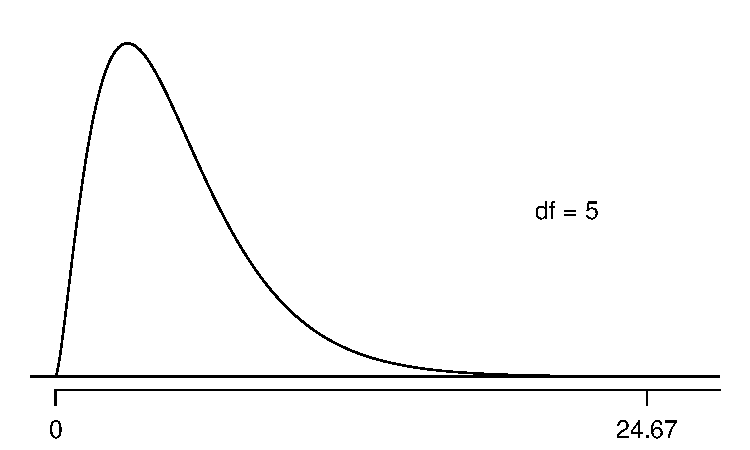
\includegraphics[width=0.67\textwidth]{6-3_chisq_gof/figures/above24Point67WithDF5/above24Point67WithDF5}
\end{center}
}
{
p値 = $P(\chi^2_{df = 5} > 24.67)$\\ は0.001未満
}

\end{frame}

%%%%%%%%%%%%%%%%%%%%%%%%%%%%%%%%%%%

\begin{frame}
\frametitle{仮説検定の結論}

\pq{p値が0.001未満と計算されました。有意水準5\%で、仮説検定の結論は何ですか？}

\begin{enumerate}[(a)]
\item $H_0$を棄却する：データはサイコロが公正であるという説得力のある証拠を提供します。
\solnMult{$H_0$を棄却する：データはサイコロに偏りがあるという説得力のある証拠を提供します。}
\item $H_0$を棄却しない：データはサイコロが公正であるという説得力のある証拠を提供します。
\item $H_0$を棄却しない：データはサイコロに偏りがあるという説得力のある証拠を提供します。
\end{enumerate}

\end{frame}

%%%%%%%%%%%%%%%%%%%%%%%%%%%%%%%%%%%

\begin{frame}
\frametitle{実は…}

\begin{itemize}

\item 1-6の軸は他の2つの軸（2-5と3-4）より一貫して短く、1の目と6の目のある面が他の面より大きいという仮説を支持しています。

\item 凹んだ点のために5と6がより頻繁に出るというピアソンの主張は、これらのデータによって支持されません。

\item カジノで使用されるサイコロはフラッシュフェースを持ち、点は周囲の素材と同じ密度のプラスチックで埋められ、精密にバランスが取られています。

\end{itemize}

\begin{center}
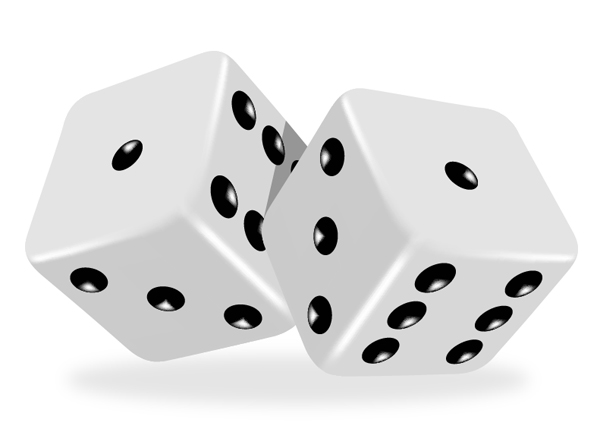
\includegraphics[width=0.3\textwidth]{6-3_chisq_gof/figures/dice/regular}
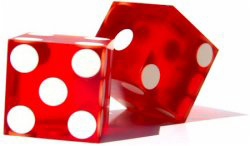
\includegraphics[width=0.3\textwidth]{6-3_chisq_gof/figures/dice/casino}
\end{center}


\end{frame}

%%%%%%%%%%%%%%%%%%%%%%%%%%%%%%%%%%%

\begin{frame}
\frametitle{まとめ：カイ二乗検定のp値}

\begin{itemize}

\item カイ二乗検定のp値は、計算された検定統計量の\hl{上の}裾の面積として定義されます。

\item 検定統計量は常に正であり、高い検定統計量ほど帰無仮説からの強い逸脱を意味するからです。

\end{itemize}

\begin{center}
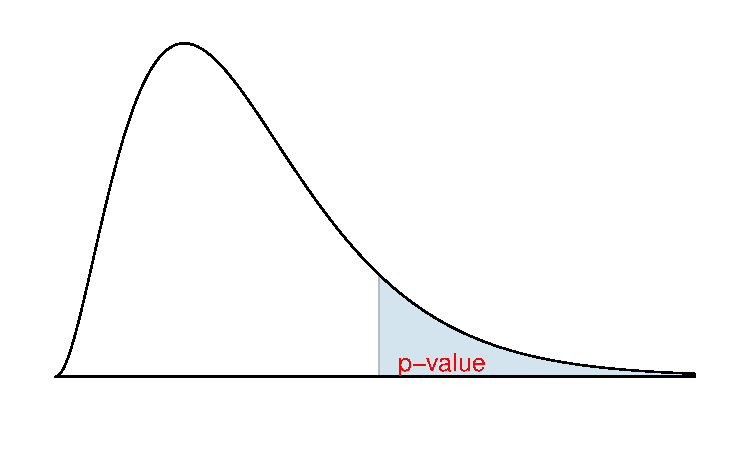
\includegraphics[width=0.7\textwidth]{6-3_chisq_gof/figures/genericChiSquare/genericChiSquare}
\end{center}

\end{frame}

%%%%%%%%%%%%%%%%%%%%%%%%%%%%%%%%%%%

\begin{frame}
\frametitle{カイ二乗検定の条件}

\begin{enumerate}

\item \hlGr{独立性：}表に度数を寄与する各ケースは、表の他のすべてのケースと独立していなければなりません。

\item \hlGr{標本サイズ：}各特定のシナリオ（すなわち、セル）は少なくとも5つの\orange{期待される}ケースがなければなりません。

\item \hlGr{$df > 1$：}自由度は1より大きくなければなりません。

\end{enumerate}

条件の確認を怠ると、意図せず検定の誤り率に影響を与える可能性があります。

\end{frame}

%%%%%%%%%%%%%%%%%%%%%%%%%%%%%%%%%%%

\subsection{2009年イラン選挙}

%%%%%%%%%%%%%%%%%%%%%%%%%%%%%%%%%%%

\begin{frame}
\frametitle{2009年イラン選挙}

\dq{2009年のイラン選挙では選挙不正が多く話題になりました。ここでは、選挙前に実施された世論調査のデータ（観測データ）と選挙で報告された得票率を比較して、両者が同じ分布に従うかどうかを確認します。}

\begin{center}
\begin{tabular}{l | r r}
					& \footnotesize{世論調査での観測} & \footnotesize{選挙での報告} \\
\footnotesize{候補者}	& \footnotesize{有権者数} & \footnotesize{得票率} \\
\hline
(1) アフマディネジャド	& 338	& 63.29\% \\
(2) ムサビ		& 136	& 34.10\% \\
(3) その他の候補者	& 30	& 2.61\% \\
\hline
合計			& 504	& 100\% \\
			& \hl{$\downarrow$}	& \hl{$\downarrow$}	\\
			& \hl{観測度数}	& \hl{期待される} \\
			& 			& \hl{分布}
\end{tabular}
\end{center}

\end{frame}

%%%%%%%%%%%%%%%%%%%%%%%%%%%%%%%%%%%

\begin{frame}
\frametitle{仮説}

\dq{報告された得票率と世論調査の分布が異なるかどうかを検定するための仮説は何ですか？}

\soln{
\begin{itemize}
\item[$H_0$:] 世論調査から観測された度数は、報告された得票率と同じ分布に従います。
\item[$H_A$:] 世論調査から観測された度数は、報告された得票率と同じ分布に従いません。
\end{itemize}
}

\end{frame}

%%%%%%%%%%%%%%%%%%%%%%%%%%%%%%%%%%%

\begin{frame}[shrink=10]
\frametitle{検定統計量の計算}

{\small
\begin{center}
\begin{tabular}{l | r r r}
				& \footnotesize{観測数} & \footnotesize{報告得票率}	& \footnotesize{期待数} \\
\footnotesize{候補者}	& \footnotesize{（世論調査）} & \footnotesize{（選挙）}		&  \footnotesize{（世論調査）} \\
\hline
\footnotesize{(1) アフマディネジャド}	& 338	& 63.29\% 	& 504 $\times$ 0.6329 = 319 \\
\footnotesize{(2) ムサビ}		& 136	& 34.10\%		& 504 $\times$ 0.3410 = 172 \\
\footnotesize{(3) その他の候補者}	& 30	& 2.61\% 		& 504 $\times$ 0.0261 = 13\\
\hline
合計			& 504	& 100\%		& 504
\end{tabular}
\end{center}
}

\begin{eqnarray*}
\tfrac{(338-319)^2}{319} &=& 1.13 \\
\tfrac{(136-172)^2}{172} &=& 7.53 \\
\tfrac{(30-13)^2}{13} &=& 22.23 \\
\chi^2_{\mathhl{df = 2}} &=& 30.89
\end{eqnarray*}


\end{frame}

%%%%%%%%%%%%%%%%%%%%%%%%%%%%%%%%%%%

\begin{frame}
\frametitle{結論}

\pq{これらの計算に基づいて、仮説検定の結論は何ですか？}

\begin{enumerate}[(a)]
\solnMult{p値が低く、$H_0$は棄却されます。世論調査から観測された度数は、報告された得票率と同じ分布に\underline{従いません}。}
\item p値が高く、$H_0$は棄却されません。世論調査から観測された度数は、報告された得票率と同じ分布に従います。
\item p値が低く、$H_0$は棄却されます。世論調査から観測された度数は、報告された得票率と同じ分布に従います。
\item p値が低く、$H_0$は棄却されません。世論調査から観測された度数は、報告された得票率と同じ分布に\underline{従いません}。
\end{enumerate}

\end{frame}
